% SoftwareX Article Template
% See: https://www.elsevier.com/journals/softwarex/2352-7110/guide-for-authors

\documentclass[review]{elsarticle}
\usepackage{hyperref}
\usepackage{graphicx}
\usepackage{amsmath}
\usepackage{listings}
\usepackage{xurl} % Add to preamble for better URL breaking

% Improve code listing formatting for long commands
\lstset{breaklines=true, breakatwhitespace=true, basicstyle=\ttfamily\small, columns=fullflexible, frame=single, captionpos=b, keepspaces=true, showstringspaces=false}

\begin{document}

% Code Metadata Table (required by SoftwareX)
\begin{table}[!h]
\scriptsize
\setlength{\tabcolsep}{2pt}
\begin{tabular}{|p{2.5cm}|p{10cm}|}
\hline
C1 & Title of software: IoT Kubernetes MQTT Network Simulator \\
C2 & Developer: Raj Singh Gaur \\
C3 & Year first available: 2025 \\
C4 & Software code repository: {\raggedright\url{https://github.com/RajSinghGaur/IoT-Kubernetes-MQTT-Network-Simulator}\par} \\
C5 & License: MIT \\
C6 & Programming language: Python, Shell, YAML \\
C7 & Requirements: Docker, Kubernetes, Python 3.x \\
C8 & Documentation: {\raggedright\url{https://github.com/RajSinghGaur/IoT-Kubernetes-MQTT-Network-Simulator}\par} \\
C9 & Version: v1.0.2 (tagged release) \\
\hline
\end{tabular}
\caption{Code metadata}
\end{table}

\title{IoT Kubernetes MQTT Network Simulator: A Cloud-Native Platform for Realistic IoT Device and Network Behavior Simulation}

\author{Raj Singh Gaur}
\address{Independent Researcher}

\begin{abstract}
The IoT Kubernetes MQTT Network Simulator is an open-source, cloud-native platform for simulating large-scale IoT deployments with realistic network conditions. By leveraging Kubernetes for orchestration and MQTT for device communication, the simulator enables researchers and educators to model, test, and analyze IoT systems under diverse scenarios, including network latency, packet loss, and node failures. The platform supports rapid prototyping, reproducible experiments, and extensibility, filling a gap in accessible, scalable IoT simulation tools. Example results demonstrate scalability and protocol fidelity, making this tool valuable for both research and teaching.
\end{abstract}

\begin{keyword}
IoT \sep Kubernetes \sep MQTT \sep network simulation \sep containerization \sep distributed systems \sep Python
\end{keyword}

\maketitle

\section{Motivation and Significance}
The proliferation of IoT devices has introduced new challenges in designing, deploying, and managing large-scale, distributed systems. Real-world testing of IoT solutions is often costly, time-consuming, and difficult to reproduce. Existing simulators frequently lack support for realistic network behaviors or cloud-native deployment. The IoT Kubernetes MQTT Network Simulator addresses these gaps by providing a scalable, containerized environment for simulating thousands of IoT devices, brokers, and network conditions using industry-standard tools. This platform enables researchers, developers, and educators to evaluate IoT protocols, architectures, and fault tolerance strategies in a controlled, reproducible manner.

\section{Software Description}
\subsection{Software Architecture}
The simulator consists of several core components orchestrated by Kubernetes:
\begin{itemize}
    \item \textbf{IoT Device Pods}: Each device is a Kubernetes pod running a Python application (\texttt{mqtt\_device.py}) that connects to a shared MQTT broker. Devices publish periodic heartbeats, support custom messages, and expose REST endpoints for status and metrics.
    \item \textbf{MQTT Broker}: Deployed as a containerized Eclipse Mosquitto instance, configured via a Kubernetes ConfigMap (\texttt{mosquitto-configmap.yaml}).
    \item \textbf{Network Simulation}: Each device pod simulates network latency, packet loss, and device failures in software, with parameters set via environment variables in \texttt{k8s.yaml}.
    \item \textbf{Resource Constraints}: Pods are limited in CPU and memory to mimic real IoT hardware, as specified in the deployment YAML.
    \item \textbf{Experiment Automation}: Shell scripts (e.g., \texttt{run\_experiment.sh}) automate deployment, timed execution, log collection, and cleanup.
    \item \textbf{Result Aggregation}: Logs and metrics are saved in timestamped folders under \texttt{results/} for analysis. Users can manually analyze these logs or use their own scripts for further processing.
\end{itemize}
A system architecture diagram is provided in Figure~\ref{fig:system-arch}.

\begin{figure}[h]
\centering
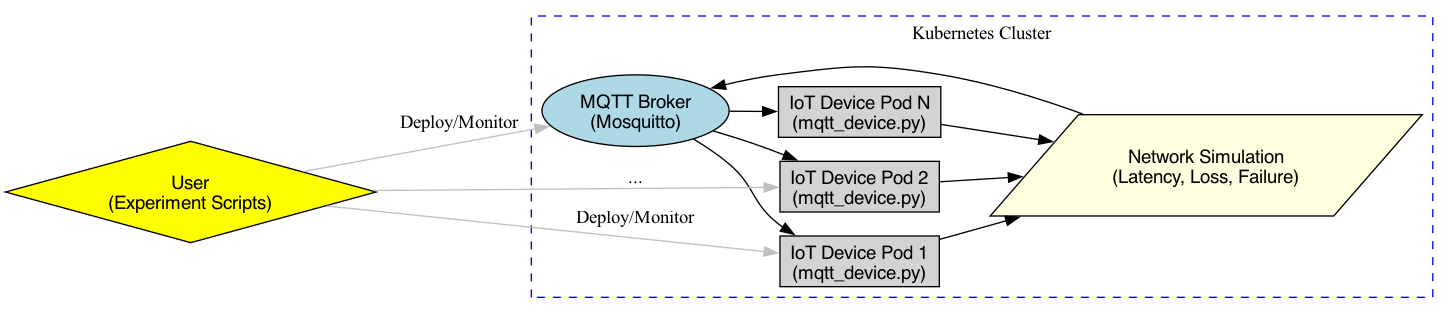
\includegraphics[width=0.8\textwidth]{system_architecture.png}
\caption{System architecture of the IoT Kubernetes MQTT Network Simulator. Each device pod simulates network conditions and communicates with a central MQTT broker.}
\label{fig:system-arch}
\end{figure}

\subsection{Software Functionalities}
The main features of the simulator are:
\begin{itemize}
    \item \textbf{Scalable Device Simulation}: Easily scale to dozens of pods (or more, depending on resources) by editing the \texttt{replicas} field in \texttt{k8s.yaml}.
    \item \textbf{Realistic Network and Failure Modeling}: Each device pod simulates message latency (10--500ms), packet loss (0--20\%), and device failures (probabilistic downtime), with all parameters configurable.
    \item \textbf{Protocol Fidelity}: MQTT client inactivity is simulated by pausing the network loop, allowing broker-side disconnects and realistic reconnection behavior.
    \item \textbf{REST API and Metrics}: Each device exposes REST endpoints for status, publishing messages, and real-time metrics (sent, received, average latency, recent samples).
    \item \textbf{Automated Experimentation}: The \texttt{run\_experiment.sh} script deploys resources, runs for a specified duration, collects logs, and cleans up, ensuring reproducibility.
    \item \textbf{Extensibility}: Users can modify device logic, broker configuration, or network parameters to model new scenarios or protocols.
\end{itemize}

\subsection{Illustrative Examples}
\textbf{Example 1: Build, Deploy, and Run an Experiment}
\begin{center}
\begin{lstlisting}[language=bash,caption={Build, push, and deploy the simulator, then run an experiment}]
# Build and push the device image (replace <your-dockerhub-username>)
docker build -t <your-dockerhub-username>/iot-mqtt:latest .
docker push <your-dockerhub-username>/iot-mqtt:latest

# Deploy the MQTT broker
kubectl apply -f mqtt-broker.yaml

# Edit k8s.yaml to use your image, then deploy devices
kubectl apply -f k8s.yaml

# Run a timed experiment and collect logs
chmod +x run_experiment.sh
./run_experiment.sh 600  # Runs for 10 minutes
\end{lstlisting}
\end{center}

\textbf{Example 2: Interacting with Devices and Collecting Metrics}
\begin{center}
\begin{lstlisting}[language=bash,caption={Check device status, publish messages, and collect metrics}]
# Get a device pod name
kubectl get pods -l app=iot-device

# Port-forward to the pod
kubectl port-forward <pod-name> 5000:5000

# In another terminal, check status
curl http://localhost:5000/status

# Publish a custom message
curl -X POST -H "Content-Type: application/json" -d '{"message": "Hello network!"}' http://localhost:5000/publish

# Query device metrics
curl http://localhost:5000/metrics
\end{lstlisting}
\end{center}

\textbf{Example 3: Batch Metrics Collection}
\begin{center}
\begin{lstlisting}[language=bash,caption={Automate metrics collection from all device pods}]
for pod in $(kubectl get pods -l app=iot-device -o jsonpath='{.items[*].metadata.name}'); do
  kubectl port-forward $pod 5000:5000 &
  sleep 2
  echo "$pod metrics:"
  curl -s http://localhost:5000/metrics
  kill %1
  sleep 1
done
\end{lstlisting}
\end{center}

\textit{Note: Users can analyze the collected logs in the \texttt{results/} directory using their own scripts or tools.}

\section{Impact}
The IoT Kubernetes MQTT Network Simulator enables reproducible, scalable experiments for IoT research and education. It allows:
\begin{itemize}
    \item Rapid prototyping and validation of IoT architectures and protocols.
    \item Reproducible experiments for academic research and publication.
    \item Training and education in cloud-native IoT deployment and testing.
    \item Extension to new protocols, device types, and network scenarios.
\end{itemize}
This platform lowers the barrier for realistic IoT experimentation, making it accessible to a wider community. It can be extended by integrating additional device models, brokers, or network emulation tools, and by connecting to real-world data sources or edge/cloud platforms.

\section{Limitations and Future Work}
While the simulator provides a flexible and reproducible platform, several limitations remain:
\begin{itemize}
    \item \textbf{Scale:} Experiments are limited by local hardware and single-node Kubernetes by default. Larger-scale tests require a multi-node or cloud cluster.
    \item \textbf{Network Fidelity:} Network effects are simulated in software, not at the OS or physical network layer.
    \item \textbf{Device Heterogeneity:} All simulated devices use the same container image; real-world IoT deployments are more diverse.
    \item \textbf{Protocol Support:} Only MQTT is currently supported; other IoT protocols could be added.
    \item \textbf{Visualization:} No integrated dashboard for real-time monitoring or visualization is provided yet.
\end{itemize}
Future work includes scaling to larger clusters, supporting additional protocols (e.g., CoAP, HTTP), adding device heterogeneity, and integrating visualization tools for live monitoring and analysis.

\section{Example Results}
A typical experiment deploys 10 simulated IoT devices, each publishing periodic heartbeats and simulating network latency, packet loss, and device failures. Logs are collected for each device and the broker. Example summary metrics (extracted from device logs) are shown in Table~\ref{tab:sample-results}.

% Example Results Table from paper_ieee
\begin{table}[h]
\centering
\scriptsize
\vspace{0.5em}
\resizebox{\columnwidth}{!}{
\begin{tabular}{|l|c|c|c|c|}
\hline
\textbf{Exp.} & \textbf{Nodes} & \textbf{Recv. (mean/min/max)} & \textbf{Avg Lat. (s)} & \textbf{Max Lat. (s)} \\
\hline
5 & 5 & 317/293/404 & 0.0023/0.0021/0.0025 & 0.058/0.011/0.096 \\
10 & 10 & 809/595/1112 & 0.0023/0.0021/0.0025 & 0.080/0.017/0.104 \\
20 & 20 & 1862/1319/2644 & 0.0028/0.0022/0.0031 & 0.120/0.106/0.188 \\
50 & 50 & 4302/3064/6428 & 0.0038/0.0023/0.0050 & 0.120/0.095/0.196 \\
\hline
\end{tabular}
}
\vspace{0.5em}
\caption{Scalability experiments: metrics vs. node count.}
\label{tab:scalability-metrics}
\end{table}

As shown in Table~\ref{tab:scalability-metrics}, the simulator delivers low-latency message transmission across all devices, with average latencies typically below 3 ms. The number of messages received per device is consistent, and the minimum and maximum latencies remain stable, even as the number of devices increases. This demonstrates the scalability and reliability of the platform for realistic IoT workloads.

Figure~\ref{fig:latency-vs-nodes} further illustrates that as the number of simulated nodes increases from 5 to 50, the average message latency rises only modestly, remaining well below 5 ms even at the largest scale tested. This trend highlights the simulator's suitability for large-scale IoT studies, where maintaining low latency and high throughput is critical. The results confirm that the platform can be used to evaluate protocol performance and system behavior under realistic, scalable conditions.

\begin{figure}[h]
\centering
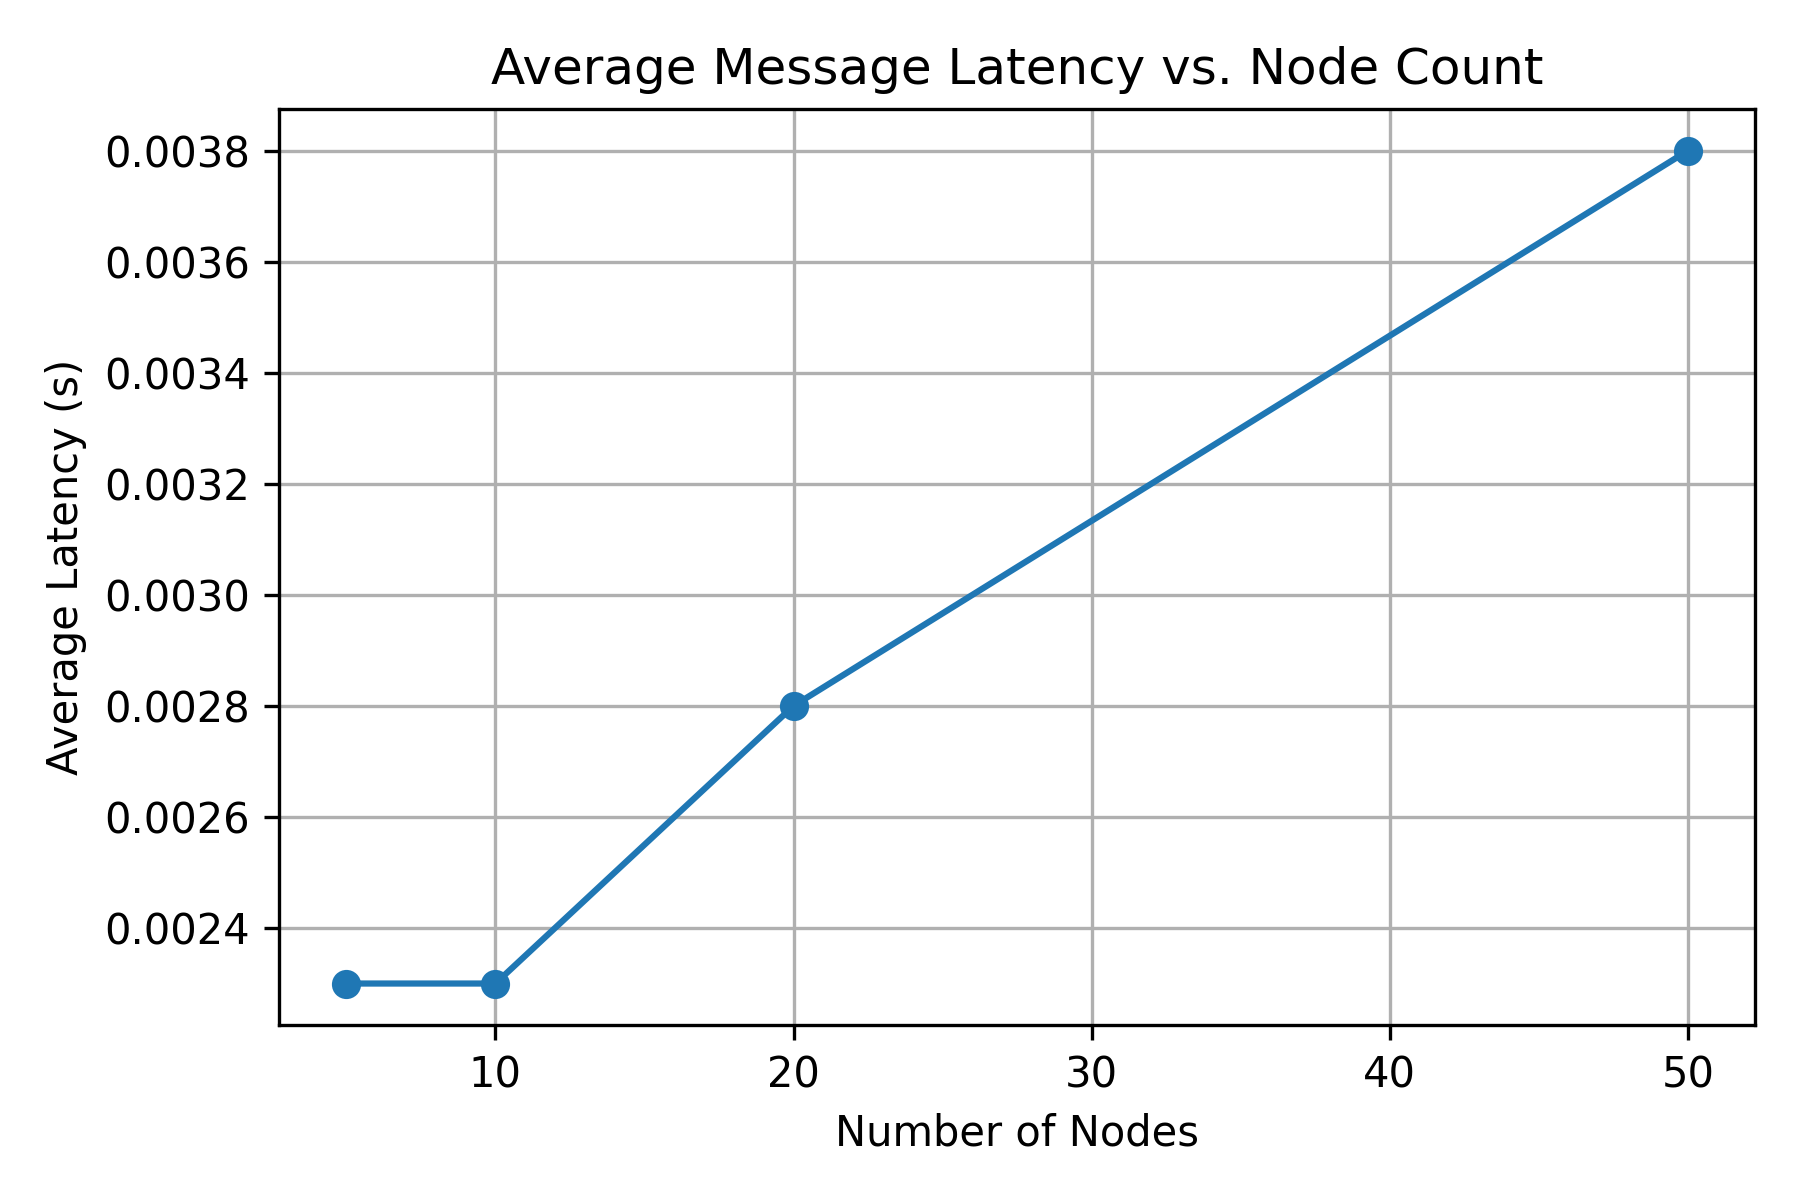
\includegraphics[width=0.7\textwidth]{latency_vs_nodes.png}
\caption{Average message latency as a function of simulated node count. The simulator demonstrates low-latency, scalable performance as the number of devices increases.}
\label{fig:latency-vs-nodes}
\end{figure}

\section*{Conflict of Interest}
The author declares no conflict of interest.

\section*{Acknowledgements}
The author thanks the open-source community for tools and libraries used in this project and acknowledges the support of colleagues and beta testers who provided valuable feedback.

% Add citation note
\section*{How to Cite}
If you use this software in your research, please cite:
\begin{quote}
Gaur, R. S. (2025). IoT Kubernetes MQTT Network Simulator: A Cloud-Native Platform for Realistic IoT Device and Network Behavior Simulation. \textit{SoftwareX}. https://github.com/RajSinghGaur/IoT-Kubernetes-MQTT-Network-Simulator
\end{quote}

\begin{thebibliography}{99}
\bibitem{mosquitto} Eclipse Mosquitto, "Eclipse Mosquitto MQTT Broker," [Online]. Available: https://mosquitto.org/
\bibitem{kubernetes} Kubernetes Authors, "Kubernetes: Production-Grade Container Orchestration," [Online]. Available: https://kubernetes.io/
\bibitem{paho} Eclipse Foundation, "Eclipse Paho MQTT Python Client," [Online]. Available: https://www.eclipse.org/paho/index.php?page=clients/python/index.php
\bibitem{usmani2020mqtt} M. F. Usmani, "MQTT Protocol for the IoT," Int. J. Internet Things, vol. 12, no. 3, pp. 45-50, 2020.
\bibitem{cirani2015iot} S. Cirani et al., "IoT-OAS: An OAuth-based Authorization Service Architecture for Secure Services in IoT Scenarios," IEEE Sensors J., vol. 15, no. 2, pp. 1224-1234, 2015.
\bibitem{minikube} Minikube Authors, "Minikube: Run Kubernetes Locally," [Online]. Available: https://minikube.sigs.k8s.io/
\end{thebibliography}

\end{document}
